\section{Noções topológicas}\index{noções topológicas}
Nessa seção, discutiremos sucintamente noções topológicas básicas sobre os espaços $\mathbb R^n$.
Ao longo dela, $n$ denota um inteiro positivo.

\subsection{Conjuntos abertos}

\begin{definition}\index{conjunto aberto}
    Seja $n\geq 1$ e seja $A$ um subconjunto de $\mathbb R^n$.
    Dizemos que $A$ é \emph{aberto} se, para todo $p\in A$, existe $r>0$ tal que $B(p, r)\subseteq A$.
\end{definition}

A intuição de conjunto aberto é a seguinte: para que $A$ seja aberto, é necessário que cada um dos seus pontos possui uma ``folga'' dentro de $A$.

\subimport{}{nocoesTopologicas-figuraAbertos}

Iniciaremos vendo que a bola aberta é aberta, justificando seu nome.

\begin{proposition}
    Sejam $n\geq 1$, $p \in \mathbb R^n$ e $r>0$.
    Então, a bola aberta $B(p, r)$ é um conjunto aberto.
\end{proposition}
\begin{proof}
    Seja $q \in B(p, r)$ arbitrário.
    Note que $d(p, q) < r$, ou seja, $\|p-q\| < r$.

    Seja $r' = r - d(p, q) > 0$.
    Veremos que $B(q, r') \subseteq B(p, r)$.

    De fato, seja $x \in B(q, r')$, ou seja, $d(q, x) < r'$.
    Então:
    \begin{align*}
        d(p, x) &\leq d(p, q) + d(q, x) \\
        &< d(p, q) + r' = d(p, q) + (r - d(p, q)) = r.
    \end{align*}

    Assim, $x \in B(p, r)$ e concluímos que $B(q, r') \subseteq B(p, r)$.

    Como $q \in B(p, r)$ foi arbitrário, concluímos que para todo $q \in B(p, r)$ existe $r'>0$ tal que $B(q, r')\subseteq B(p, r)$.

    \begin{figure}[H]
    \centering
    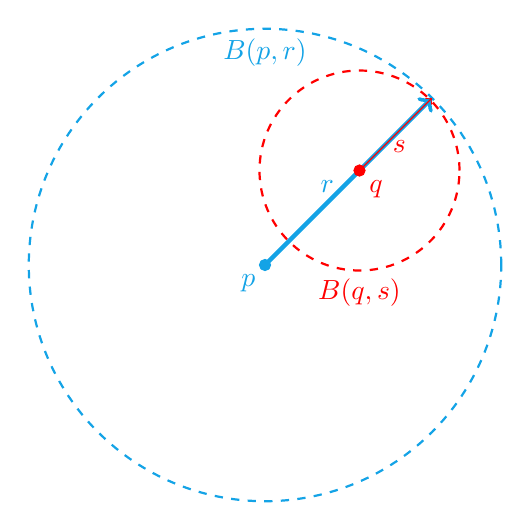
\begin{tikzpicture}
    % Bola B(p, r)
    \draw[thick, dashed, Cerulean] (0,0) circle (3);
    \filldraw[Cerulean] (0,0) circle (2pt) node[below left] {$p$};
    \node[Cerulean] at (0,2.7) {$B(p, r)$};
    % Raio r
    \draw[ultra thick,Cerulean,->] (0,0) -- (2.12,2.12);
    \node[Cerulean, left] at (1,1) {$r$};

    % Bola B(q, s)
    \filldraw[Red] (1.2,1.2) circle (2pt) node[below right] {$q$};
    \draw[thick, dashed, Red] (1.2,1.2) circle (1.27);
    \node[Red] at (1.2,-0.35) {$B(q, s)$};
    % Raio s
    \draw[Red,->] (1.2,1.2) -- (2.12,2.12);
    \node[Red, right] at (1.5,1.5) {$s$};

    % Relação de inclusão
    \end{tikzpicture}
    \caption{Relação de inclusão entre as bolas abertas.}
    \end{figure}
\end{proof}

Algumas propriedades básicas dos conjuntos abertos são as seguintes.

\begin{proposition}\index{conjunto aberto!propriedades}
    Sobre abertos de $\mathbb R^n$, temos as seguintes propriedades.
    \begin{enumerate}[label=(\roman*)]
        \item $\mathbb R^n$ e o conjunto vazio $\emptyset$ são abertos.
        \item A união de qualquer coleção de conjuntos abertos é aberta.\index{conjunto aberto!união}
        \item A interseção de dois conjuntos abertos é aberta.\index{conjunto aberto!interseção finita}
    \end{enumerate}
\end{proposition}
\begin{proof}
    (i) O conjunto $\mathbb R^n$ é aberto porque, para todo $p \in \mathbb R^n$, temos que $B(p, 1) \subseteq \mathbb R^n$.
    O conjunto vazio $\emptyset$ é aberto por vacuidade: do contrário, haveria um ponto $p \in \emptyset$ tal que, para todo $r>0$, $B(p, r)\not\subseteq \emptyset$, o que é absurdo, pois não existem pontos no conjunto vazio.

    (ii) Seja $\{A_i\}_{i \in I}$ uma coleção indexada de conjuntos abertos de $\mathbb R^n$.
    Seja $A = \bigcup_{i \in I} A_i$.
    Seja $p \in A$ arbitrário.
    Então, existe $j \in I$ tal que $p \in A_j$.
    Como $A_j$ é aberto, existe $r>0$ tal que $B(p, r) \subseteq A_j\subseteq A$, e, portanto, $B(p, r) \subseteq A$.
    Assim, $A$ é aberto.

    (iii) Seja $A_1$ e $A_2$ conjuntos abertos de $\mathbb R^n$.
    Seja $p \in A_1\cap A_2$ arbitrário.
    Existe $r_1>0$ tal que $B(p, r_1) \subseteq A_1$ e existe $r_2>0$ tal que $B(p, r_2) \subseteq A_2$.
    Seja $r = \min\{r_1, r_2\}$.
    Então, $B(p, r) \subseteq B(p, r_1) \subseteq A_1$ e $B(p, r) \subseteq B(p, r_2) \subseteq A_2$, ou seja, $B(p, r) \subseteq A_1\cap A_2$.
    Assim, $A_1\cap A_2$ é aberto.
\end{proof}
\subimport{}{nocoesTopologicas-figuraIntersecaoAbertos}

\begin{knowMore}
    Um \emph{espaço topológico} é, por definição, um par $(X, \tau)$, em que $X$ é um conjunto e $\tau$ é uma coleção de subconjuntos de $X$ tal que:
    \begin{enumerate}[label=(\roman*)]
        \item $X$ e $\emptyset$ pertencem a $\tau$;
        \item A união de qualquer coleção de conjuntos pertencentes a $\tau$ pertence a $\tau$;
        \item A interseção de dois conjuntos pertencentes a $\tau$ pertence a $\tau$.
    \end{enumerate}
    Nesse contexto, os conjuntos pertencentes a $\tau$ são chamados de \emph{conjuntos abertos} de $X$.
    Assim, pela proposição anterior a definição de espaço topológico é uma generalização da noção de conjunto aberto que vimos para $\mathbb R^n$.
\end{knowMore}

\begin{example}\label{exemplo:intervalos-abertos-sao-abertos}
    Em $\mathbb R$, intervalos abertos $]a, b[$ com $a<b$ são conjuntos abertos.
    Para ver isso, podemos escrevê-lo como uma ``bola'' aberta.
    
    Seu ponto médio, $x=\frac{a+b}{2}$, é um candidato natural a ser o centro da bola aberta.

    Para acharmos um candidato a raio, primeiro vamos medir a distância entre $x$ e $a$.
    Temos que $d(x, a) = \left|\frac{a+b}{2} - a\right| = \frac{b-a}{2}$.
    Assim, seja $r = \frac{b-a}{2}$.

    Afirmo que $]a, b[=B(x, r)$.

    Com efeito, dado $c \in \mathbb R$, temos que:
    \begin{align*}
        c \in B(x, r) &\Leftrightarrow d(c, x) < r \\
        &\Leftrightarrow |c-x| < r \\
        &\Leftrightarrow |c-\frac{a+b}{2}| < \frac{b-a}{2} \\
        &\Leftrightarrow -\frac{b-a}{2} < c-\frac{a+b}{2} < \frac{b-a}{2} \\
        &\Leftrightarrow a-b< 2c - a - b < b-a \\
        &\Leftrightarrow a-b+(a+b) < 2c < b-a+(a+b) \\
        &\Leftrightarrow 2a< 2c < 2b \\
        &\Leftrightarrow a < c < b \\
        &\Leftrightarrow c \in ]a, b[.
    \end{align*}

    Assim, $]a, b[=B(x, r)$ é um conjunto aberto.
\end{example}

\subimport{}{nocoesTopologicas-figuraIntervalosAbertos}

\begin{example}
    O intervalo aberto $]a, +\infty[\subseteq \mathbb R$, com $a \in \mathbb R$, é um conjunto aberto.
    
    Para ver isso, basta notar que $]a, +\infty[ = \bigcup_{b>a} ]a, b[$ é uma união de conjuntos abertos, logo é aberto.

    Analogamente, o intervalo aberto $]-\infty, a[$ é um conjunto aberto.
    De fato, $]-\infty, a[ = \bigcup_{b<a} ]b, a[$ é uma união de conjuntos abertos, logo é aberto.
\end{example}

\subsection{Pontos isolados e de acumulação de subconjuntos de $\mathbb R^n$}

A noção de ponto isolado captura a ideia de que um ponto de um conjunto é ``separado'' dos outros pontos do conjunto.
Há uma ``folga'' em torno dele que o separa dos outros pontos do conjunto.

\begin{definition}\index{ponto isolado}
    Seja $n\geq 1$ e seja $A$ um subconjunto de $\mathbb R^n$.
    Dizemos que um ponto $p \in A$ é um \emph{ponto isolado} de $A$ se existe $r>0$ tal que $B(p, r)\cap A = \{p\}$.
\end{definition}

\begin{example}
    Em $\mathbb R^2$, seja $A = B(0, 1)\cup \{(2, 0)\}$ 
    Temos que $p=(2, 0)$ é um ponto isolado de $A$, logo $f$ é contínua em $(2, 0)$.
    De fato, considere $r=1$.
    
    Temos que $B(p, r)\cap A=\{p\}$.
    Com efeito, temos que $p\in B(p, r)\cap A$, pois $p \in A$ e $d(p, p) = 0 < r$.
    Reciprocamente, se $x \in B(p, r)\cap A$, temos que $x\notin B(0, 1)$, pois se $x \in B(0, 1)\cap B(p, r)$, então $d(0, p) \leq d(0, x) + d(x, p) < 1 + r = 2$, assim, $d(0, p)<2$.
    Por outro lado, $d(0, p)=\sqrt{(2-0)^2 + (0-0)^2} = \sqrt{4} = 2$, o que é uma contradição.
\end{example}

\subimport{}{nocoesTopologicas-figuraExemploPontoIsolado}

Um ponto de acumulação de um subconjunto $A$ de $\mathbb R^n$ é, intuitivamente, um ponto que está ``grudado'' nos pontos de $A$ diferentes dele próprio.

\begin{definition}\index{ponto de acumulação}
    Seja $n\geq 1$ e seja $A$ um subconjunto de $\mathbb R^n$.
    Dizemos que um ponto $p \in \mathbb R^n$ é um \emph{ponto de acumulação} de $A$ se, para todo $r>0$, o conjunto $B(p, r)\cap A\setminus\{p\}$ é não vazio.
\end{definition}

A expressão $B(p, r)\cap A\setminus\{p\}\neq\emptyset$ significa que em $B(p, r)\cap A$, existe um ponto diferente de $p$.

Ou seja, independente de quão pequeno seja um raio $r$ dado, teremos um ponto de $A$ diferente de $p$ que dista de $p$ menos de $r$.

\subimport{}{nocoesTopologicas-figuraPontoAcumulacao}


Como um primeiro exemplo, veremos que os pontos de abertos de $\mathbb R^n$ são pontos de acumulação do aberto em questão.

\begin{proposition}\label{prop:abertosPontosAcumulacao}
    Seja $n\geq 1$ e seja $A$ um subconjunto aberto de $\mathbb R^n$.

    Então todo ponto de $A$ é um ponto de acumulação de $A$.
\end{proposition}
\begin{proof}
    Seja $A$ um conjunto aberto de $\mathbb R^n$ e seja $p \in A$ arbitrário.
    Como $A$ é aberto, existe $r>0$ tal que $B(p, r)\subseteq A$.

    Dado $s>0$, queremos ver que $B(p, s)\cap A\setminus\{p\}\neq \emptyset$.

    Seja $s'=\min\{s, r\}$.
    Temos que:

    \begin{align*}
        B(p, s)\cap B(p, r)=&\{x \in \mathbb R^n : d(p, x) < s\} \cap \{x \in \mathbb R^n : d(p, x) < r\} \\=& \{x \in \mathbb R^n : d(p, x) < \min\{s, r\}\}\\=& B(p, \min\{s, r\})=B(p, s').
    \end{align*}

    Assim, temos que $B(p, s')=B(p, s)\cap B(p, r)\subseteq B(p, s)\cap A$.

    Basta ver, então, que $B(p, s')$ possui pontos diferentes de $p$.
    Daremos uma prova formal para esse fato ``visualmente intuitivo'' (recomenda-se tentar desenhar, caso tenha dificuldades em visualizar o desejado).

    De fato, consideremos exemplo um pequeno deslocamento de $p$ na direção $e_1=(1, 0, \dots, 0)$, ou seja, considere $q=p+\delta e_1$ para algum $\delta > 0$ que será escolhido a seguir. Temos que
    \[
    d(q, p) = \|q-p\| = \|p+\delta e_1 - p\| = \|\delta e_1\| = \delta\|e_1\| = \delta.
    \]

    Tomando $\delta=\dfrac{s'}{2}$, temos que $d(q, p) = \delta < s'$, ou seja, $q \in B(p, s')$.
\end{proof}

\subimport{}{nocoesTopologicas-figuraAbertosPontosAcumulacao}

Pontos isolados e de acumulação são, em algum sentido, antagônicos.

\begin{proposition}\index{ponto isolado!ponto de acumulação}
    Seja $n\geq 1$, seja $A$ um subconjunto de $\mathbb R^n$ e seja $p \in A$.
    
    Então uma, e apenas uma das seguintes afirmações é verdadeira:
    \begin{enumerate}[label=(\roman*)]
        \item $p$ é um ponto isolado de $A$;
        \item $p$ é um ponto de acumulação de $A$.
    \end{enumerate}
\end{proposition}
\begin{proof}
    (i) e (ii) não podem valer simultaneamente:
    a primeira afirmação diz que existe $r>0$ tal que $B(p, r)\cap A = \{p\}$.
    Mas, então, para esse mesmo $r>0$, temos que $B(p, r)\cap A\setminus\{p\} = \emptyset$, o que é uma contradição com a segunda afirmação.

    Para ver que uma delas deve valer, vamos supor que não vale (ii) e mostrar que (i) segue.
    Como (ii) não vale, existe $r>0$ tal que $B(p, r)\cap A\setminus\{p\} = \emptyset$.
    Veremos que $B(p, r)\cap A = \{p\}$.

    De fato, temos que $p \in B(p, r)\cap A$, pois $p \in A$ e $d(p, p) = 0 < r$.
    Reciprocamente, se $x \in B(p, r)\cap A$, temos que $x=p$, do contrário, teríamos que $x \in B(p, r)\cap A\setminus\{p\}$, o que é uma contradição.
\end{proof}

Temos ainda que pontos de acumulação são ``indestrutíveis'' pela remoção de um número finito de pontos.

\begin{proposition}\label{proposicaoPontoAcumulacaoRemocaoPontos}
    Seja $n\geq 1$, seja $A$ um subconjunto de $\mathbb R^n$ e seja $p \in \mathbb R^n$ um ponto de acumulação de $A$.

    Então, para todo conjunto finito $F\subseteq \mathbb R^n$, o ponto $p$ é um ponto de acumulação de $A\setminus F$.
\end{proposition}
\begin{proof}
    Seja $F$ um conjunto finito de $\mathbb R^n$ e seja $s>0$ arbitrário.

    Devemos ver que $\big(B(p, s)\cap (A\setminus F)\big)\setminus\{p\}\neq \emptyset$.

    Para cada $a \in F\setminus\{p\}$, seja $r_a = d(p, a)$.
    Seja $r = \min(\{s\}\cup\{r_a : a \in F\setminus\{p\}\})$.
    Temos que cada $r_a=d(p, a)$ é positivo, pois $a\neq p$.
    Assim, $r>0$.

    Como $p$ é um ponto de acumulação de $A$, temos que $B(p, r)\cap A\setminus\{p\}\neq \emptyset$.
    Seja $x \in B(p, r)\cap A\setminus\{p\}$ arbitrário.

    Temos que $x\in B(p, r)\subseteq B(p, s)$, pois $r\leq s$.

    Temos que $x\notin F$, pois, dado $a \in F$, temos que $d(p, a)=r_s\geq r$, e $d(p, x)<r$.

    Assim, $x \in B(p, s)\cap (A\setminus F)\setminus\{p\}$.

    Portanto, $\big(B(p, s)\cap (A\setminus F)\big)\setminus\{p\}\neq \emptyset$.
\end{proof}

Daí, o seguinte corolário é imediato.
\begin{corollary}
    Seja $n\geq 1$, seja $A$ um subconjunto aberto de $\mathbb R^n$.
    Se $F$ é finito, então todo ponto de $A$ é um ponto de acumulação de $A\setminus F$.
\end{corollary}
\begin{proof}
    Seja $p \in A$ arbitrário.
    Como $A$ é aberto, $p$ é um ponto de acumulação de $A$.
    Como $F$ é finito, $p$ ainda é um ponto de acumulação de $A\setminus F$ pela proposição anterior.
\end{proof}

\subsection{Subconjuntos fechados de $\mathbb R^n$}

Intuitivamente, um conjunto fechado é um conjunto que contém todos os seus pontos que estão ``grudados'' nele.

\begin{definition}\index{conjunto fechado}
    Seja $n\geq 1$ e seja $A$ um subconjunto de $\mathbb R^n$.
    Dizemos que $A$ é \emph{fechado} se, para todo ponto de acumulação $p$ de $A$, temos que $p \in A$.
\end{definition}

Uma forma frequentemente mais prática de verificar se um conjunto é fechado é o seguinte critério.
\begin{proposition}
    Seja $n\geq 1$ e seja $A$ um subconjunto de $\mathbb R^n$.
    Então, $A$ é fechado se, e somente se, seu complemento $\mathbb R^n\setminus A$ é aberto.
\end{proposition}

\begin{proof}
    Primeiramente, suponha que $A$ é fechado.
    Veremos que $\mathbb R^n\setminus A$ é aberto.

    Seja $p \in \mathbb R^n\setminus A$ arbitrário.
    O ponto $p$ não é um ponto de acumulação de $A$, pois, caso contrário, como $A$ é fechado, teríamos que $p \in A$, o que é uma contradição.

    Assim, como $p$ não é ponto de acumulação de $A$, existe $r>0$ tal que $B(p, r)\cap A\setminus\{p\} = \emptyset$.
    Daí, $B(p, r)\cap A\subseteq \{p\}$.
    Como $p \notin A$, temos que $B(p, r)\cap A = \emptyset$.
    Dessa forma, $B(p, r)\subseteq \mathbb R^n\setminus A$.

    Reciprocamente, suponha que $\mathbb R^n\setminus A$ é aberto.
    Veremos que $A$ é fechado.
    Para tanto, devemos ver que para todo $p\in \mathbb R^n$, se $p$ é um ponto de acumulação de $A$, então $p \in A$.
    Pela contrapositiva, basta ver que para todo $p\in \mathbb R^n$, se $p \notin A$, então $p$ não é um ponto de acumulação de $A$.

    De fato, dado $p \in \mathbb R^n\setminus A$, como $\mathbb R^n\setminus A$ é aberto, existe $r>0$ tal que $B(p, r)\subseteq \mathbb R^n\setminus A$, de modo que $B(p, r)\cap A = \emptyset$.
    Assim, $B(p, r)\cap A\setminus\{p\} = \emptyset$, o que mostra que $p$ não é um ponto de acumulação de $A$.
\end{proof}

\begin{example}
    O intervalo $[a, b]$ com $a<b$ é um conjunto fechado de $\mathbb R$, pois $\mathbb R\setminus [a, b] = ]-\infty, a[ \cup ]b, +\infty[$ é uma união de conjuntos abertos, logo é aberto.
\end{example}

\begin{corollary}
    Seja $n\geq 1$ e seja $A$ um subconjunto de $\mathbb R^n$.
    Então, $A$ é aberto se, e somente se, seu complemento $\mathbb R^n\setminus A$ é fechado.
\end{corollary}
\begin{proof}
    Seja $B=\mathbb R^n\setminus A$.
    Temos que $B$ é aberto se, e somente se, $\mathbb R^n\setminus B$ é fechado.
    Mas $\mathbb R^n\setminus B = \mathbb R^n\setminus (\mathbb R^n\setminus A) = A$.
    Assim, $B=\mathbb R^n\setminus A$ é aberto se, e somente se, $\mathbb R^n\setminus B = A$ é fechado.
\end{proof}

\begin{proposition}
    Seja $n\geq 1$ e seja $F$ um subconjunto de $\mathbb R^n$.
    Então $F$ não possui pontos de acumulação.
    Em particular, $F$ é fechado.
\end{proposition}
\begin{proof}
    Temos, pela Proposição~\ref{proposicaoPontoAcumulacaoRemocaoPontos} aplicado com $A=F$, que se $p$ é um ponto de acumulação de $F$, então $p$ é um ponto de acumulação de $F\setminus F=\emptyset$.

    Assim, basta notar que o conjunto vazio $\emptyset$ não possui pontos de acumulação.
    De fato, seja $p \in \mathbb R^n$ arbitrário e seja $r>0$.
    Temos que $B(p, r)\cap \emptyset\setminus\{p\} = \emptyset$.

    Para a última afirmação, temos que $F$ não possui pontos de acumulação, logo, por vacuidade, todo ponto de acumulação de $F$ pertence a $F$ (do contrário, haveria um ponto de acumulação de $F$ que não pertence a $F$, o que é uma contradição, pois $F$ não possui pontos de acumulação).
\end{proof}

\begin{proposition}
    Seja $n\geq 1$, seja $A$ um subconjunto de $\mathbb R^n$ e seja $C$ um subconjunto fechado de $\mathbb R^n$.
    Então $A\setminus C$ é um conjunto aberto de $\mathbb R^n$.
\end{proposition}
\begin{proof}
    De fato, temos que $A\setminus C = A\cap(\mathbb R^n\setminus C)$ é uma interseção de dois conjuntos abertos, logo, é aberto.
\end{proof}
